% .:: Laden der LaTeX4EI Formelsammlungsvorlage
\documentclass[fs, footer]{latex4ei}


\usepackage{listings}
\usepackage{hyperref}


% Dokumentbeginn
% ======================================================================
\begin{document}


% Aufteilung in Spalten
\vspace{-4mm}
\begin{multicols*}{4}
	\fstitle{Internet-kommunikation}
% -------------------------------------------
% | 		Internetkommunikation			|
% ~~~~~~~~~~~~~~~~~~~~~~~~~~~~~~~~~~~~~~~~~~~
% SECTION ====================================================================================
\textbf{Hinweis:} Im Fach 'Internetkommunikation' ist in der Klausur keine Formelsammlung zugelassen. Daher kann diese Formelsammlung lediglich zur Prüfungsvorbereitung dienen.

\sectionbox{
\section{Das Internet}
% ============================================================================================
„Ein Netz aus Netzen“ – Öffentliches Internet verbindet private Intranets.\\
\subsection{Begriffe}

\tablebox{
	\begin{tabular*}{\columnwidth}{@{\extracolsep\fill}rl@{}} \ctrule

		User & Teilnehmer \\
		Terminal & Endgerät \\
		Router & \\
		Nodes & \\
		Links & Abschnitte \\
		M2M & Maschine zu Maschine \\
		MSS & Maximum Segment Size\\
		RTT & Round Trip Time\\
	\cbrule
	\end{tabular*}
}
\subsection{Netzstrukturen}
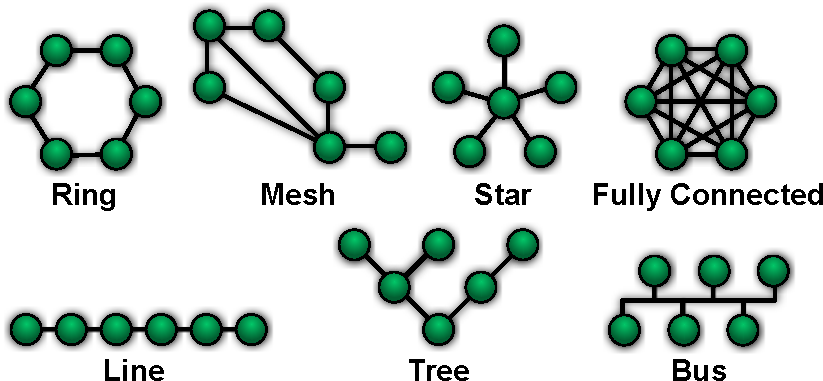
\includegraphics[width= \columnwidth]{./img/net_topologies.pdf}


\subsection{Architekturen}
\begin{description}
	\item[Client/Server:] Ständige Verfügbarkeit
	\item[Peer to Peer(P2P):] Hohe Skalierbarkeit, da jeder Besitzer auch Anbieter einer Datei ist.
\end{description}
\paragraph{Paketvermittlung} (100 – 1000 Byte)
Pakete teilen sich die Netzressourcen, statistisches Multiplexen.
Ermöglicht varaible Übertragungsraten
\paragraph{Routing} bestimmt den Weg von Quelle zur Senke.
\paragraph{Forwarding} Eingehende Pakete werden an den richtigen Ausgang geleitet.

}

\sectionbox{
	\subsection{Kommunikation}
	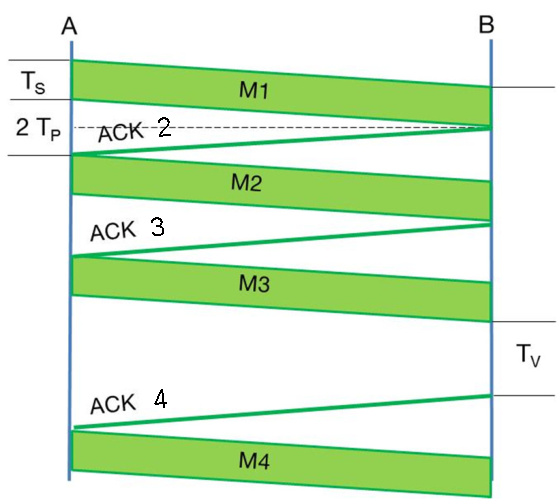
\includegraphics[width = 5cm]{./img/comm.pdf}


}



\vfill
% SECTION ====================================================================================
\section{Protokolle (Regeln)}
% ============================================================================================
Protokolle definieren das Format und die Reihenfolge in der Nachrichten im System gesendet und empfangen werden.

\sectionbox{
\subsection{OSI-ISO Schichtenmodell}

	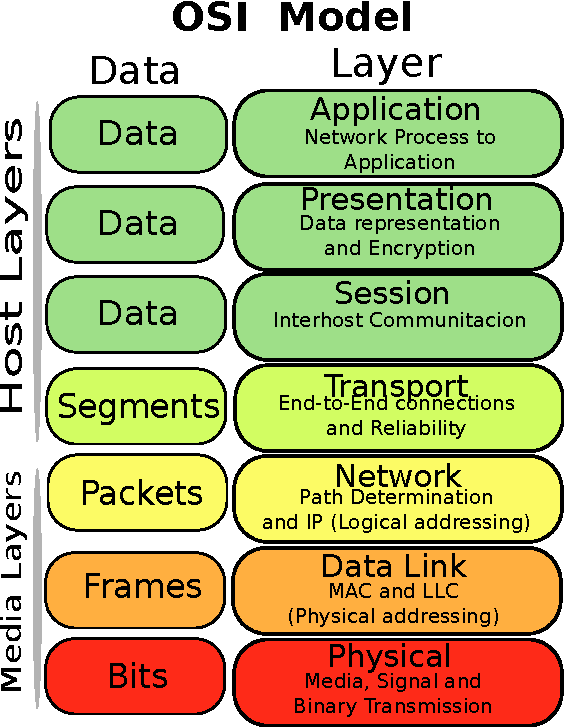
\includegraphics[height=5cm]{img/Osi-model.pdf}
}
\sectionbox{

\subsection{Internet Layers}
\symbolbox{
	\begin{tabular*}{\columnwidth}{ll}
		$T_{\ir s}$ & Übertragungsverzögerung
	\end{tabular*}
}
\begin{description}
		\item[Application (HTTP:)] Regelt Syntax und Semantik von Nachrichten
		\item[Transport (TcCP):] Ende-zu-Ende Datentransfer zwischen Prozessen.
		\item[Network (IP):] Routing der Pakete durchs Netz mit Quell- und Zieladresse.
		\item[Link (MAC,LLC):] Verteilung des Medienzugangs (MAC) und Sicherung der Übetragung durch Flusssteuerung (LLC) mit Prüfsummen.
		\item[Physical (PHY):] Bits auf der Leitung/el. magn. Welle
\end{description}

Kenngrößen eines Netzwerks:
	\begin{description}
		\item[Delay (Verzögerung):] und Jitter, d.h. Schwankung der Verzögerung\\
			$T_{\ir ges} = \underset{\text{Verarbeitung}}{T_{\ir VK}} + \underset{\text{Wartezeit Puffer}}{T_{\ir VQ}} + \underset{\text{Übertragung}}{T_{\ir S}} + \underset{\text{Ausbreitung}}{T_{\ir P}}$\\
			$T_{\ir S} = \frac{L}{R} = \frac{\text{Packetgröße (Bit)}}{\text{ Bandbreite einer Leitung (Bit/s)}}$

			$T_{\ir P} = \frac{d}{s} = \frac{\text{Leitungslänge}}{\text{Ausbreitungsgeschwindigkeit}}$
		\item[Loss (Verlust:)] Verluste von Paketen
		\item[Throughput (Durchsatz:)] $R \cdot \rho$ \qquad Goodput: $R \cdot \rho \frac{L_{\ir D}}{L_{\ir H} + L_{\ir D}}$\\
			Leitung mit kleinstem $R$ begrenzt den Throughput (Engpass)
		\item[Verkehrsauslastung:] $\eta = \text{Anforderungsrate} \cdot \text{Verzögerung} = a \cdot T_{\ir S}$
\end{description}


}
\sectionbox{
	\subsection{Kendall Notation für Warteschlangen}
	Kendall Notation: X / Y / N / s / q\\
	\\
	\symbolbox{
		\begin{tabular}{ll}
				X & Art des Ankuftsprozesses (M für Markov)\\
				Y & Art des Bedienprozesses (M für Markov)\\
				N & Anzahl der Bedieneinheiten (Server)\\
				s & Kapazität (Plätze) der Warteschlange\\
					& Verlustsystem $s=0$, Wartesystem $s \ra \infty$\\
					& Warteverlustsystem $0 < s < \infty$\\
				q & Zahl der Quellen\\
				$\lambda_X$ & Geburtsrate\\
				$\mu_{\X}$ & Sterberate\\
		\end{tabular}
	}

	Wartewahrscheinlichkeit $\P_{\ir W}$ dafür, dass ein ankommendes Paket warten muss, also falls Pakete $> N$

	Mittlere Warteschlangenlänge $\Omega = p_N \frac{\frac{A}{N}}{\left(1-\frac{A}{N}\right)^2}$\\
	Mittlere Wartezeit $T_{\ir W} = \frac{\Omega}{\lambda}$\\
	Angebot: $A = \frac{\lambda}{\mu}$ \qquad Ausnutzung:$\rho = \frac{A}{N} = 1 - p_0$\\
	\\
	Protokoll Wirkungsgrad $\rho = \frac{T_{\ir S}}{T_{\ir S} + 2 T_{\ir P}}$ \qquad (Für stop \& wait)\\
	Nachrichtensendedauer $T_{\ir S}$; Kanallaufzeit $T_{\ir P} = \frac{l}{c}$

	\subsubsection{Poisson-Prozess}
		Geburtsrate $\lambda = \frac{1}{E [A]}$

	\subsubsection{Neg-Exponentialverteilung}
		mittlere Bearbeitungszeit (Sterberate) $\mu = \frac{1}{\text{Bedienzeit}}$
}
\sectionbox{
	\subsection{Flusssteuerung}
	Go-back-N: Übertragene P bei Fehler: $\mathrm{Time} - 2 T_{\ir P} - t_{\ir out} + 1$\\
	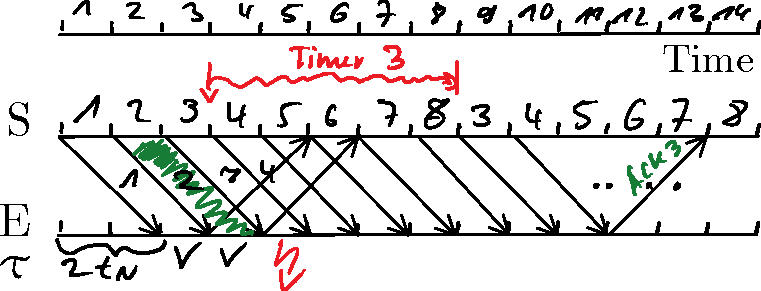
\includegraphics[width = \columnwidth]{./img/fluss.pdf}

}
\section{Protokolle (Beispiele)}

\sectionbox{
\subsection{HTTP}
\texttt{\noindent
GET /somedir/page.html HTTP/1.1\\
Host: www.someschool.edu\\
User-agent: Mozilla/4.0\\
Header-Zeilen Connection: close\\
Accept-language:fr}


	\subsubsection{Allgemein}
	Non-Persistent: Neue Anfrage für jedes Objekt (2 RTT pro Objekt)\\
	Persistent: Server lässt Verbindung offen (1 RTT pro Objekt)\\
	Pipelining: Parallele Object Requests möglich ($\approx$ 1 RTT für alles)\\
	DNS Anfrage: $T_{\ir DNS} = RTT$, \qquad TCP Aufbau: $T_{\ir TCP} = RTT$\\

	Gesamtladen $T_{\ir HTTP} = 2 RTT + 4 T_{\ir Si}$\\
	Round-Trip-Time $RTT = 2(T_{\ir p} + T_{\ir v})$\\
	$T_{\ir Si} = T + T +T $\\

	\subsubsection{Coockies}
	\begin{enumerate}
		\item set-cookie: Kopfzeile in der HTTP Response Nachricht\\
		\item Cookie Kopfzeile in jeder HTTP Request Nachricht\\
		\item Cookie auf dem Rechner des Anwenders\\
		\item Cookie in der Datenbank des Servers\\
	\end{enumerate}


	\subsubsection	{Web-Cache}
	Benutzer definiert Webzugriff über Cache (Proxy-Server)\\
	Browser sendet alle HTTP-Requests an den Cache\\
	Im Cache: Proxy sendet Seite aus dem Cache an den Client\\
	Nicht im Cache: Proxy läd Seite in den Cache und leitet sie weiter\\
}
\sectionbox{
\subsection{FTP – File Transfer Protocol}
	Client kontaktiert Server: \\
	Login:   user: <name>, pass: <password> \\
	Dateizugriff:  list, retr <file>, stor <file>

}
\sectionbox{

\subsection{SMTP – Simple Mail Transfer Protocol [RFC 822]}

Header:  To: <adress>, From: <adress>, Subject: <subject>  \\
Zugriffsprotokolle: POP3 [RFC 1939], IMAP [RFC 1730], HTTP\\

}
\sectionbox{
\subsection{DNS – Domain Name System}
Übersetzung von Hostnamen zu IP Adressen\\
Kanonische Namen (Originalname) oder Aliase (Alternativnamen)\\
Baumstruktur: DNS-Rootserver speichert TLD-DNS-Server (org, com)\\
Iterativ: Client $\ra$ Lokaler DNS $\ra$ Rest der Reihe nach probieren\\
Rekursiv: Client $\rightleftarrows$ Lokaler DNS $\rightleftarrows$ RootDNS $\rightleftarrows$ TLD-DNS\\
}

\section{Transportschicht}

Ende-zu-Ende Transport zwischen Prozessen auf hosts
\begin{itemize}
	\item 2 Tupel $\ra$ UDP
	\item 4 Tupel $\ra $ TCP
\end{itemize}

zuverlässige Übertragung

\subsection{Fensterprotokoll}

Kanalausnutzung $\rho_n = \frac{L_N}{L} \frac{W_s t_n}{t_R}$

\subsection{IP – Internet Protocol}



\sectionbox{
	\subsubsection{UDP – User Datagram Protocol [RFC 768]}
	Unzuverlässiger Transport

	Minimales, best-effort

	2 Tupel: Empfänger IP, Empfänger Port

	--- Bild UDP mit Sockets ---
}
\sectionbox{
	\subsubsection{TCP – Transfer Control Protocol Reno [RFC 793]}
	Zuverlässige Datenübertragung

	--- Bild TCP mit Sockets ---

	4 Tupel:  Empfänger IP, Empfänger Port, Sender IP, Sender Port\\
	\\
	Zustände:\\
	\textbf{Server:} \texttt{CLOSED, LISTEN, SYN\_RECV, ESTB, CLOSE\_WAIT, LAST\_ACK}\\
	\textbf{Client:} \texttt{CLOSED, SYN\_SENT, ESTB, FIN\_WAIT1, FIN\_WAIT2, TIME\_WAIT}

	\textbf{Header:}

	Max-Sequenznummer: $2^{32}$ Bit

	\textbf{Three-Way-Handshake}
	%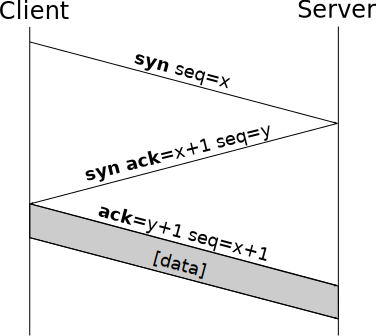
\includegraphics{./img/Tcp-handshake.svg}

	\textbf{FlowControl:} Sender schickt nicht mehr Daten als Empf. puffern kann.\\
	\textbf{ACK:} Empfänger bestätigt jedes Packet mit einem \texttt{ACK} + \texttt{seq} vom nächsten erwarteten Paket. Ist das nächste anders $\ra$ duplicated \texttt{ACK}\\
	\textbf{Fast-Retransmit:} Falls 3 \texttt{Ack} mit selber \texttt{seq} $\ra$ resend before timeout\\
	\textbf{Three-Way-Handshake:} \texttt{SYN} $\ra$ \texttt{SYN+ACK} $\ra$ \texttt{ACK}\\

	\textbf{Fehlererkennung} Timer (wird bei Empfang eines \texttt{ACK}s zurückgesetzt) oder 3 gleiche \texttt{ACK}s $\ra$ fast retransmit

	\textbf{Congestion Control:} Verhindert Überlastung: $\texttt{Rate} = \frac{\texttt{CongWin}}{\texttt{RTT}}$\\
	Slowstart: Exp. Wachstum (Verdopplung pro \texttt{RTT}) von \texttt{CongWin}, ab \texttt{thresh} lineares Wachstum. (+1\texttt{MSS} pro \texttt{RTT}) \\
	Bei 3 doppelten \texttt{Ack}s: \texttt{threshNew} = \texttt{CongWinNew} = \texttt{CongWin/2} (Reno)\\
	Bei Timeout/Anfang: \texttt{CongWinNew} = 1, \qquad \texttt{threshNew} = \texttt{CongWin/2}\\
	\\
	LastByteSent - LastByteAcked $\le$ CongWin

	\symbolbox{
	\begin{tabular}{cc}
	    $L$ & Fehlerrate \\
		$W$ & max. Fenstergröße
	\end{tabular}

	}
	\textbf{Durchsatz:} $D = \frac{\text{Daten}}{\text{Zeit}} = \frac{1.22 \cdot \texttt{MSS}}{\texttt{RTT} \cdot \sqrt{L}} = \frac{0,75 \cdot N \cdot \texttt{MSS}}{\texttt{RTT}} = \frac{0,75 \cdot W}{\texttt{RTT}}$


MSS (Max. Seg. Size.) = MTU - Header IP - Header TCP $\approx 1500 \si{Byte}$

$R = \frac{W \cdot  MSS}{RTT}$ \\

durchschnittliche Fenstergröße mit cong. control: $\frac{W + \frac W 2}{2} = 0.75 W$

Anzahl der Segmente die einen Link voll ausnutzen:

%$ \#_s = \frac{R \cdot \texttt{RTT}{MSS}$
}

\subsection{Protokolle auf verlustbehafteten Kanälen}

Wirkungsgrad (Utilization):

$U = \frac{\text{Nachrichten Sendedauer}}{\text{Zeit bis nächste Nachricht gesendet werden kann}} = \frac{T_s}{RTT + T_s}$

\subsection{Protokolle mit Pipelining}
Prinzip: Sende mehrere unbestätigte Pakete und warte dann auf ACKs.

Puffern der unbestätigten Pakete notwendig, höhere Sequenznummern.

\subsubsection{Go-Back-N}

--- Bild Go-Back-N (aus Folie) ---



Schiebe Sendefenster bei entpsr. \texttt{ACK} um eins über die Pakete.
Nur ein Timer für das gesamte Fenster. Wenn Timer abläuft, sende gesamtes Fenster nochmals.


\subsubsection{Selective Repeat}

Wiederhole nur Pakete für die keine ACKs empfangen wurden.
\subsection{Anwendungsschicht} % (fold)
\label{sub:anwendungsschicht}

--- Bild ---



\paragraph{Prinzipien} % (fold)
\label{par:prinzipien}

\begin{tabular}{ll}
	Architektur: & Client-Server / P2P\\
	Overlay: & virtuelle Netzstruktur\\
	Adressierung & Host(IP) + Port\\
	Transportdienstgüte: & Delay / Loss / Durchsatz\\
	Info-Abruf: & pull/push\\
	Nachrichtenformat & \\
	Zustand & stateless / stateful\\
	Verbindungsverwaltung & persistent / non-persistent\\
\end{tabular}




% ==============================================================================================
\section{Netzschicht}
% ==============================================================================================
Protokolle: IP, ATM\\
Aufgaben: Routing und Forwarding\\
IP: BestEffort, Reihenfolge egal,  keine Zuverlässigkeit\\

	\subsection{Router}
	Routing: Memory, Bus, Crossbar\\
	\\
	Pufferdimensionierung bei $N$ Datenflüssen und Link-Datenrate $R$\\
	Puffergröße $P = \frac{\texttt{RTT} \cdot R}{\sqrt{N}}$\\


	\subsection{IP -- Internet Protocol [RFC]}
	\noindent IPv4:\\
	\indent \quad\ 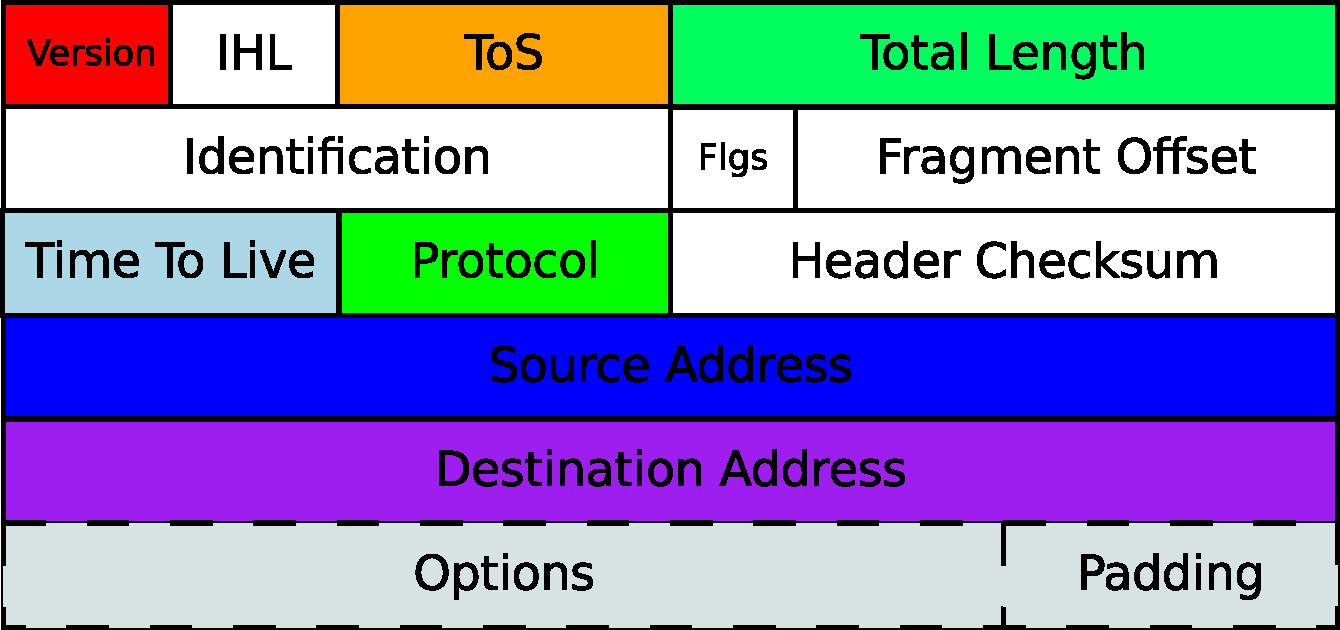
\includegraphics[width = 5cm]{./img/IPv4_header.pdf} \\
	IPv6:\\
	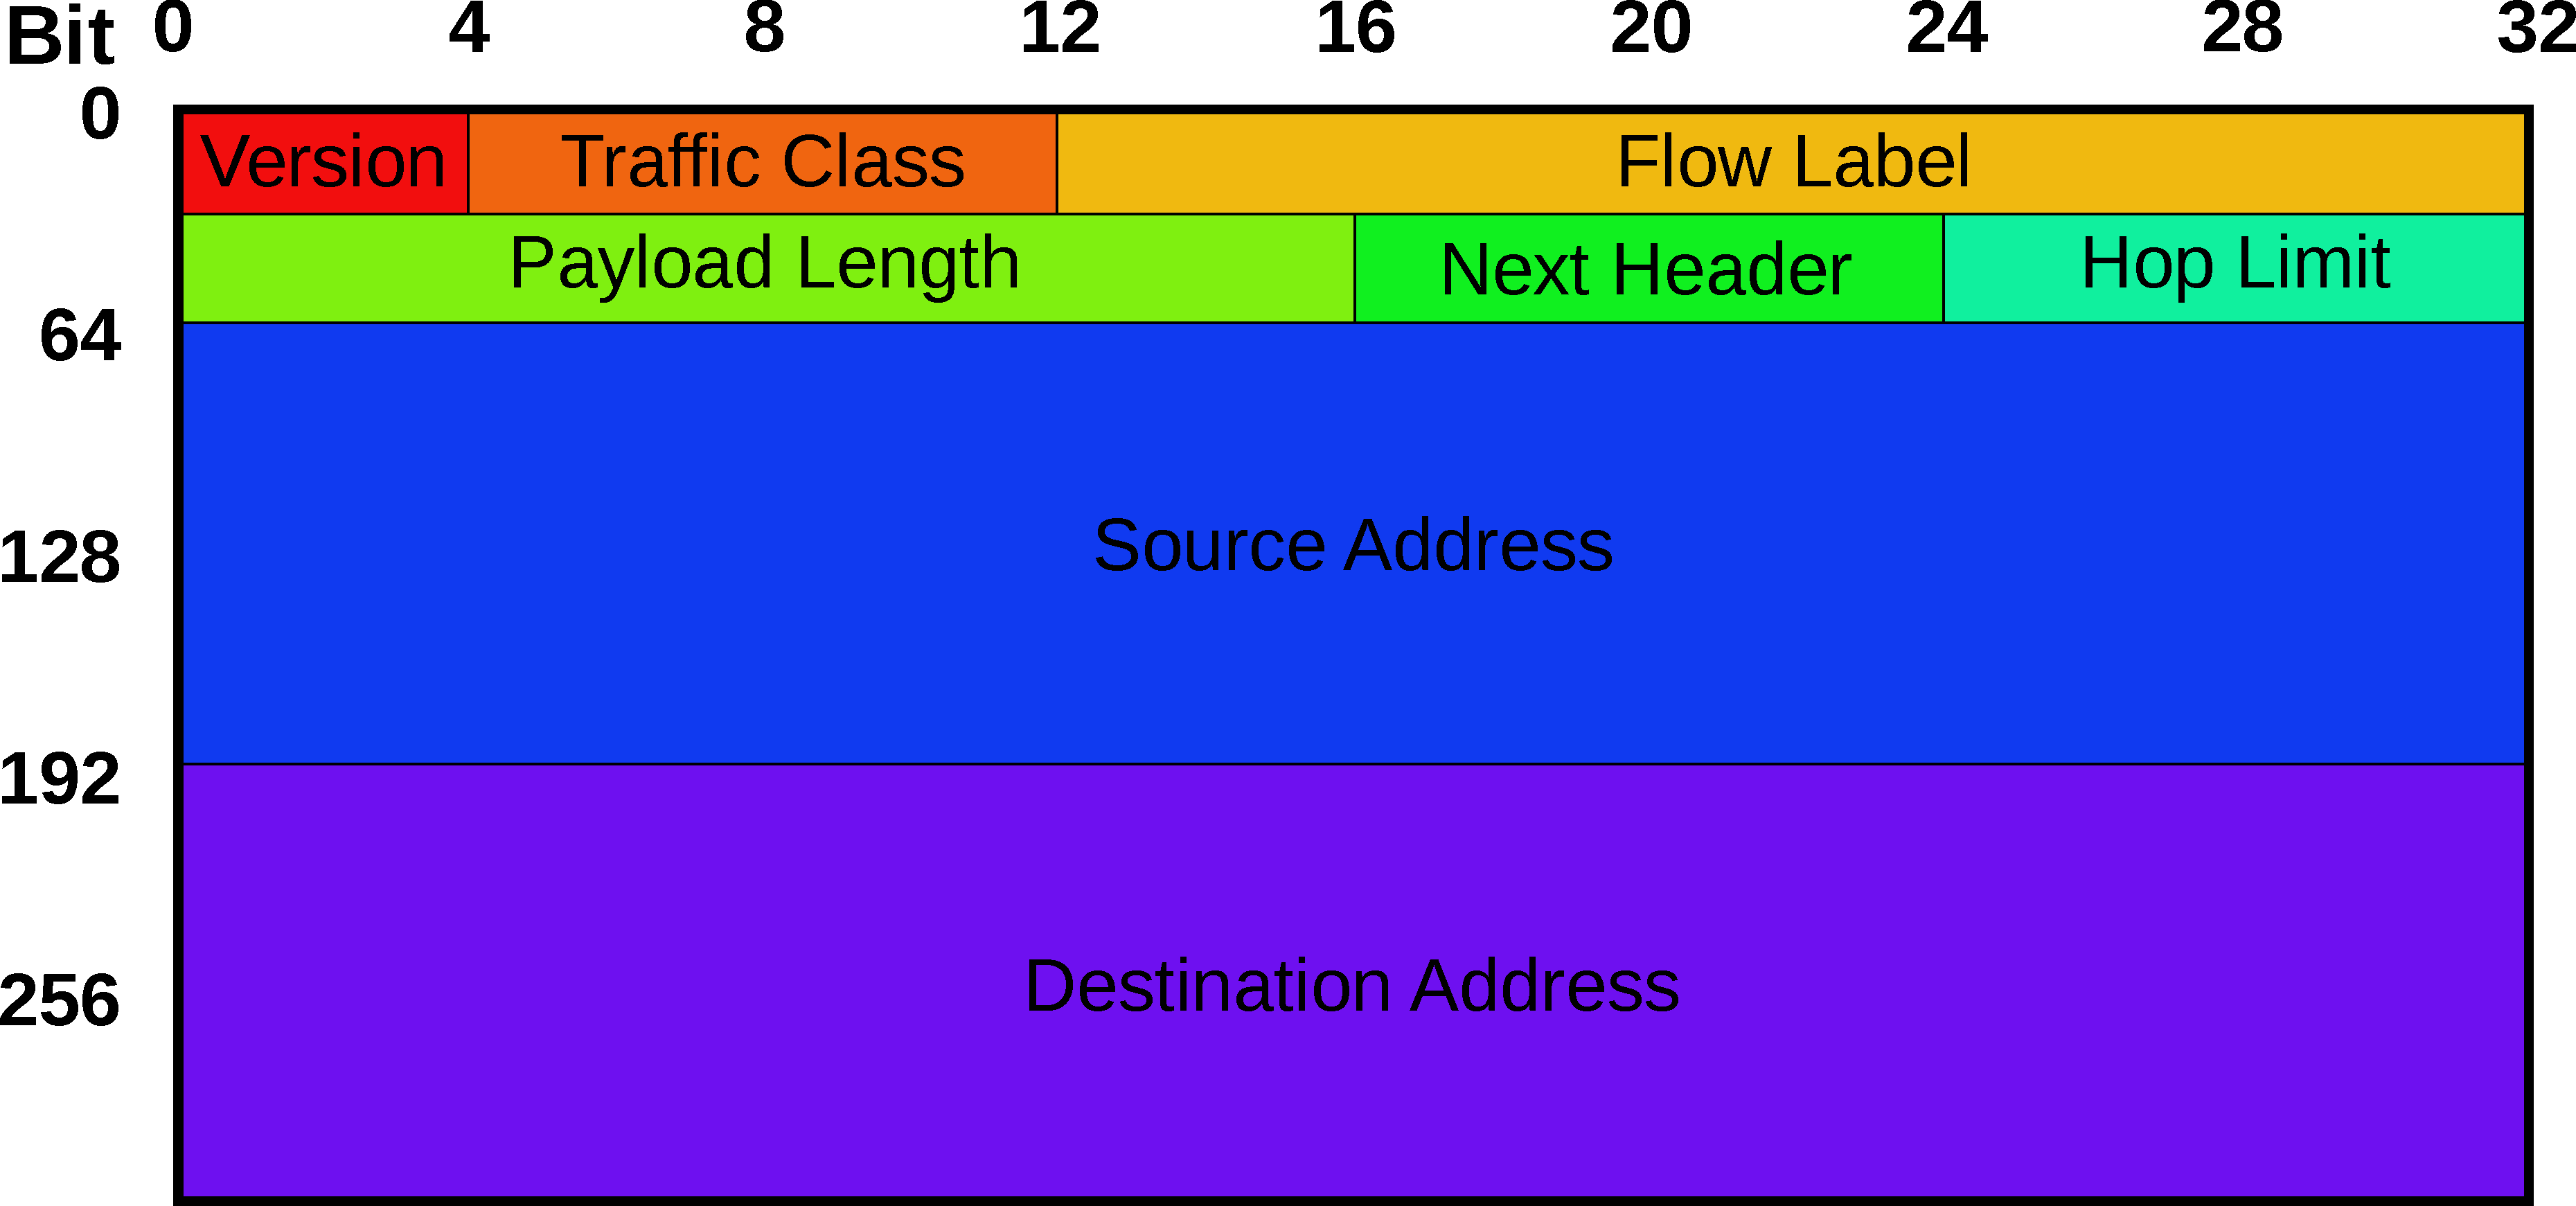
\includegraphics[width = 5.5cm]{./img/IPv6_header.pdf} \\

	20 Byte Header
	Seit 1993: Klassenlose Adressierung

		\subsubsection{Abbildung auf MAC-Adressen}
		\begin{tabular}{lll}
		Version & Protocol & Table\\ \mrule
		IPv4 & Address Resolution Protocol ARP & ARP-Table\\
		IPv6 & Neighbor Discovery Protocol NDP & NDP-Table\\
		\end{tabular}

		\subsubsection{DHCP -- Dynamic Host Configuration Protocol [RFC 2131]}
		Automatische Vergabe von Adressen und Parametern über UDP ohne manuelle Konfiguration

		\subsubsection{NAT -- Network Adress Translation}
		Abbildung von verschiedenen LAN Adressen auf eine WAN Adresse mit unterschiedlichen Ports.

		\subsubsection{Subnetze}
		200.56.168.0/21 bedeutet von $32 \si{bit}$ sind $21 \si{bit}$ fest und $32-21 = 11 \si{bit}$ variabel\\
		\\
		Anzahl der Class C Subnetze (/24): $24-21 = 3$ \quad $2^{3} = 8$\\
		Anzahl der IP-Adressen: $32 - 21 = 11$ \quad $2^{11} = 2048$


	\subsection{IPv6}
	32 Bit Adresse, 40 Byte Header, Verkehrsklassen für QoS\\
	Migration mit Tunneling (IPv6 im Datenteil von IPv4)\\

	\subsection{ICMP -- Internet Control Message Protocol [\href{https://tools.ietf.org/html/rfc792}{RFC 792}]}
	Für Pings und Fehler

	\subsection{Routingverfahren}
	Dijkstra Algorithmus (erfordert globales Wissen)\\
	globale Infornation: Link-State-Routing\\
	jeder Knoten berechnet den kürzesten Weg zu jedem anderen Router\\
	\\
	dezentrale (lokale) Information: Distance-Vector-Routing\\
	Jeder Knoten schätzt den kürzesten Weg zu jedem anderen Router\\
	\\
	Hirachisches Routing Autonomer Systeme AS:\\
	Inter-AS-Routing: BGP -- Border Gateway Protocol [RFC 4271]\\
	BGP hält das Internet zusammen!\\
	Intra-AS-Routing: RIP, OSPF, IGRP\\



% ==============================================================================================
\sectionbox{
	\section{Quality of Service}

		\subsection{Prinzipien}
		\begin{enumerate}
			\item Markieren(Verkehrsklassen) und differenziert weiterleiten:\\
				Scheduling Algorithmen: FIFO, Priority, Round Robin, WFQ\\
			\item Isolation = Eingrenzung und Überwachen: Policing/Shaping $\ra$
					\emph{Token Bucket} begrenzt Paketfluss auf vorgegebene Burst-Größe und vorgegebene durchschnittliche Rate. \\
					max. Pakete $\le R \cdot t$ und $\le b + r \cdot t$
			\item Ressourcen vollständig ausnutzen
			\item \emph{Admission Control}: Datenfluss meldet Bedarf und muss ggf. abgewiesen werden
		\end{enumerate}


	\begin{description}
		\item[DiffServ] verschiedene Klassen priorisieren den Verkehr (Feld in IP)
		\item[IntServ] Reservierung auf dem gesamten Pfad (Garantie mit RSVP)
	\end{description}



	Weighted Fair Queuing:
	$B_i = \frac{W_i}{\sum_{j=1}^{n} W_j} \cdot R$ \qquad Gewichtung $W$

	Delay Weighted Fair Queuing + Token Bucket:\\
	$d_{\ir max, WFQ} = \frac{b_i}{R w_i / \sum w_j}$\\
	$d_{\ir max, TB} = \frac{b_i (R- S_i)}{S_i(R - r_i) w_i / \sum w_j}$\\

	$w_i$: Prioritätsgewicht des Kanals, $R:$ Gesamtrate, $b:$ max Anzahl der Tokens
	$r:$ Tokenrate, $S:$ Warteschlangenrate
}

% ==============================================================================================
\section{Link Layer and Medium Access Control}
% ==============================================================================================
Transportiert \emph{frames} von einem Knoten über einen \emph{Link} zum Nachbarknoten. Regelt Zugriff auf das Medium (MAC)\\
Protokolle: Ethernet, WLAN, PPP

Frame: In header(MAC-Adresse) und trailer(Checksum) verpacktes Datagramm\\
Fehler durch Signalabfall und Rauschen\\

	\subsection{Medium Access Control}
	\begin{description}
		\item [Aufteilung des Mediums] (Partitioning): Datenrate aufteilen in Zeit/Frequenz
		\item [Wahlfreier Zugriff] (Random Access): Kollisionenserkennung: Nur senden wenn Kanal frei
		\item [Abwechselnder Zugriff]
	\end{description}
	\emph{Exponential Backoff:} Zufällige Wartezeit aus einem exponentiell steigenden Zeitbereich
	ARP um MAC Adresse über Broadcast ermitteln.


	Hub: Verbindet bloß alle Kabel, keine Pufferung\\
	Switch: Pufferung, gezielte Weiterleitung



% Prüfung: Kein Warteverlustsystem, Ü-Aufgabe 5+6 kombiniert
% Vermutlich kein Routing (Aufgabe 18)
% Aufgabe8: Abwandlungen möglich: Senden aufhören, gesammelte ACKs etc... -> Aufmerksam lesen!

% sresch-hould

% ==============================================================================================
\section{Sonstiges}
% ==============================================================================================

\begin{tabular*}{\columnwidth}{@{\extracolsep\fill}llll@{}} \trule
Port & Service & Protocols & Description \\ \mrule
20 & ftp-data & TCP/UDP & File Transfer Data\\
21 & ftp & TCP/UDP & File Transfer Control\\
22 & ssh & TCP & SSH Remote Login Protocol\\
23 & telnet & TCP & Telnet \\
25 & smtp & TCP & Simpler Mail Transfer Protocol\\
53 & domain & TCP/UDP & Domain Name Server\\
80 & http & TCP & Hypertext Transfer Protocol\\
110 & pop3 & TCP & Post Office Protocol 3\\
143 & imap4 & TCP & Interner Message Access Protocol 4\\
443 & ssl & TCP & HTTPS: HTTP over TLS/SSL\\ \brule
\end{tabular*}



% Ende der Spalten
\end{multicols*}

% Dokumentende
% ======================================================================
\end{document}

% ToDos:

